% !TeX root = relatorio.tex
\documentclass[12pt,a4paper]{article}

\usepackage[T1]{fontenc}
\usepackage[utf8]{inputenc}
\usepackage[brazilian]{babel}
\usepackage{lmodern}
\usepackage[a4paper,margin=2.5cm]{geometry}
\usepackage{amsmath}
\usepackage{amssymb}
\usepackage{graphicx}
\usepackage{float}
\usepackage{booktabs}
\usepackage{hyperref}
\usepackage{xcolor}

\hypersetup{
  colorlinks=true,
  linkcolor=blue,
  urlcolor=blue,
  pdftitle={Relatorio do Trabalho 2},
  pdfauthor={Gustavo Shoiti Sonoda}
}
\urlstyle{tt}

\renewcommand{\contentsname}{Sumário}
\setlength{\parindent}{0pt}
\setlength{\parskip}{0.7em}
\linespread{1.05}

\newcommand{\arquivo}[1]{\nolinkurl{#1}}
\newcommand{\campo}[2]{\textbf{#1.} #2\par}
\newcommand{\figdir}[1]{figuras/#1}

\begin{document}
\hypersetup{pageanchor=false}
\pagenumbering{gobble}

\begin{titlepage}
  \centering

  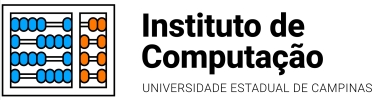
\includegraphics[width=0.24\textwidth]{figuras/logo_ic.png}\par
  \vspace{0.8cm}
  {\large Universidade Estadual de Campinas\par}
  {\large Instituto de Computação\par}

  \vspace{1.5cm}

  {\Large \textbf{Relatório de Implementação do Trabalho 2}\par}
  \vspace{0.5cm}
  {\large Introdução ao Processamento Digital de Imagens (MC920/MO443)\par}
  \vspace{1.2cm}

  {\large Relatório de implementação desenvolvido para a disciplina\\
    Introdução ao Processamento Digital de Imagens.\par}

  \vspace{1.5cm}

  \begin{flushleft}
    \textbf{Professor:} Hélio Pedrini\\
    \textbf{Aluno:} Gustavo Shoiti Sonoda\\
    \textbf{RA:} 217579\\
  \end{flushleft}

  \vfill

  Campinas -- São Paulo\\
  \today
\end{titlepage}

\tableofcontents
\newpage
\hypersetup{pageanchor=true}
\pagenumbering{arabic}

% ---------------------------------------------------------------------------
\section{Introdução}
% ---------------------------------------------------------------------------

O Trabalho 2 da disciplina MC920/MO443 propõe a implementação e análise de dois grupos de
técnicas de processamento digital de imagens e vídeo: métodos de segmentação por
limiarização (global e local) e métodos de detecção de transições abruptas em vídeos.
A vetorização de comandos foi empregada sempre que pertinente.

A Seção~\ref{sec:limiarizacao} descreve os nove métodos de binarização: limiar global fixo,
Otsu, Bernsen, Niblack, Sauvola e Pietaksinen, Phansalskar et al., Contraste, Média e
Mediana. As entradas são imagens monocromáticas no formato PGM provenientes do diretório
\url{http://www.ic.unicamp.br/~helio/imagens_pgm/}; as saídas são imagens binárias em PNG.
A Seção~\ref{sec:video} apresenta os três detectores de transições em vídeo baseados em
diferenças entre pixels, blocos e histogramas, aplicados a vídeos MP4.

% ---------------------------------------------------------------------------
\section{Materiais e Métodos}
% ---------------------------------------------------------------------------

\subsection{Ambiente e organização}

\campo{Linguagem e bibliotecas}{A implementação foi desenvolvida em Python~3. O projeto
utiliza \textit{Pillow} para leitura e gravação de imagens PGM/PNG, \textit{NumPy} nas
operações vetorizadas e \textit{SciPy} (\texttt{scipy.ndimage}) para filtros deslizantes.
A leitura de vídeos MP4 é feita com \textit{OpenCV} (\texttt{cv2}).
\textit{Matplotlib} gera os histogramas e os gráficos de métricas de vídeo.
A infraestrutura comum de preparação de entradas e geração de saídas é centralizada em
\arquivo{src/common/}.}

\campo{Organização dos arquivos}{O código do Trabalho~2 está em
\arquivo{src/trabalho\_02/}, subdividido em \arquivo{secao\_01/} (métodos de limiarização)
e \arquivo{secao\_02/} (detecção em vídeo). As entradas de cada método ficam em
\arquivo{data/input/trabalho\_02/secao\_XX/metodo\_XX/}, os resultados em
\arquivo{results/trabalho\_02/secao\_XX/metodo\_XX/},
os benchmarks em \arquivo{results/benchmarks/trabalho\_02/secao\_XX/metodo\_XX/} e as figuras
do relatório em \arquivo{docs/relatorio\_02/figuras/secao\_XX/metodo\_XX/}.}

\campo{Imagens utilizadas}{Foram processadas as sete imagens PGM disponíveis no servidor do
professor: \textit{baboon}, \textit{fiducial}, \textit{monarch}, \textit{peppers},
\textit{retina}, \textit{sonnet} e \textit{wedge} (todas com resolução $512\times 512$ pixels,
exceto \textit{fiducial}, que é $640\times 480$). Para os métodos de vídeo utilizou-se o
arquivo \texttt{lisa.mpg}.}

\campo{Representação das imagens}{Imagens monocromáticas foram tratadas como arrays NumPy
de inteiros em $[0,255]$. As saídas binárias seguem a convenção do enunciado: pixel com
valor maior que o limiar é classificado como objeto (preto, valor~0); os demais são
rotulados como fundo (branco, valor~255).}

\subsection{Benchmarks e integração com o relatório}

\campo{Medição de desempenho}{Os tempos foram coletados para cada método usando a imagem
\textit{baboon} ($512\times 512$), com 5~repetições e 1~execução de aquecimento (métodos de
vídeo: 3~repetições). Em cada método foi comparada a implementação com laços Python com a
alternativa vetorizada em NumPy/SciPy. Os resultados são resumidos na
Tabela~\ref{tab:benchmark}.}

\campo{Figuras do relatório}{As imagens mostradas ao longo do texto foram copiadas de
\arquivo{results/} para \arquivo{docs/relatorio\_02/figuras/} pelo script
\arquivo{build\_report.py}, garantindo sincronização entre os resultados gerados e o PDF
compilado.}

\subsection{Tabela comparativa de desempenho}

\begin{table}[H]
\centering
\caption{Tempos médios de execução (imagem $512\times 512$, 5~repetições).}
\label{tab:benchmark}
\begin{tabular}{lrrl}
\toprule
\textbf{Método} & \textbf{Loop (ms)} & \textbf{Vetorizado (ms)} & \textbf{Ganho} \\
\midrule
Global              &    3{,}2  &   5{,}1  & \textit{overhead NumPy} \\
Otsu                &    6{,}0  &   4{,}9  & 1{,}2$\times$ \\
Bernsen             &  530{,}1  &  17{,}0  & 31$\times$ \\
Niblack             & 1979{,}0  &  13{,}2  & 150$\times$ \\
Sauvola             & 2006{,}7  &  14{,}2  & 141$\times$ \\
Phansalskar         & 2069{,}2  &  14{,}1  & 147$\times$ \\
Contraste           &  576{,}3  &  18{,}9  & 30$\times$ \\
Média               &  548{,}0  &   9{,}6  & 57$\times$ \\
Mediana             & 2285{,}1  & 417{,}5  & 5{,}5$\times$ \\
\midrule
Pixels (vídeo)      & 4859{,}2  &  23{,}2  & 209$\times$ \\
Blocos (vídeo)      &  482{,}5  &  63{,}2  & 7{,}6$\times$ \\
Histogramas (vídeo) & 1733{,}8  & 149{,}1  & 11{,}6$\times$ \\
\bottomrule
\end{tabular}
\end{table}

% ---------------------------------------------------------------------------
\section{Métodos de Limiarização Global e Local}
\label{sec:limiarizacao}
% ---------------------------------------------------------------------------

O objetivo desta parte é implementar e analisar métodos de limiarização global e local em
imagens monocromáticas. Métodos globais determinam um único valor de limiar para toda a
imagem; métodos adaptativos locais calculam um limiar individual para cada pixel com base
na informação contida em uma vizinhança. Em ambos os casos, se o valor de $p(x,y)$ for maior
que o limiar, o pixel é classificado como objeto (preto); caso contrário, é rotulado como
fundo (branco). Para cada método são apresentados o histograma da \textbf{imagem
binarizada} (duas barras em 0 e 255, com as frações de pixels pretos e brancos indicadas)
e o limiar utilizado. Para métodos locais, o limiar anotado é a média espacial do mapa de
limiares calculado pixel a pixel.

% ---------- 1.1 Global ------------------------------------------------------
\subsection{Método Global}

\campo{Enunciado}{Se o valor de intensidade de um pixel $(x,y)$ for maior do que um limiar
$T$ (por exemplo, $T=128$), o pixel será considerado como pertencente ao objeto; caso
contrário, será considerado como fundo.}

\campo{Abordagem escolhida}{A binarização foi aplicada com \texttt{np.where}: pixels com
valor $> T$ recebem 0 (objeto/preto); os demais recebem 255 (fundo/branco). O limiar fixo
utilizado foi $T = 128$.}

\campo{Opções de vetorização}{A comparação pixel a pixel é naturalmente mapeável em
\texttt{np.where(arr > T, 0, 255)}, que opera sobre todo o array de uma só vez. A versão
com laços Python percorre $H \times W$ iterações explícitas; a versão NumPy delega a
comparação e atribuição ao núcleo C interno.}

\campo{Benchmark}{Conforme a Tabela~\ref{tab:benchmark}, a versão em laços Python executa
em $3{,}2$\,ms enquanto a vetorizada leva $5{,}1$\,ms. O overhead da versão NumPy se deve
ao custo de criação do array de saída e da chamada de função: para operações simples como
esta, o tempo de processamento é dominado pela alocação de memória e não pelo cálculo em si.}

\campo{Discussão}{O limiar fixo $T=128$ é o método mais simples e rápido, mas depende
fortemente da distribuição de intensidades da imagem. Imagens com histograma bimodal
bem definido (como \textit{wedge}) produzem boas separações; imagens com distribuição
ampla (como \textit{baboon} ou \textit{monarch}) geram resultados genéricos. A fração de
pixels pretos varia consideravelmente entre as imagens — de $\sim$30\% em imagens claras
(como \textit{retina}) a $\sim$65\% em imagens escuras.}

\begin{figure}[H]
  \centering
  \begin{minipage}{0.32\textwidth}
    \centering
    \includegraphics[width=\linewidth]{\figdir{secao_01/metodo_01_global}/global_baboon_original.png}
    \caption*{Original}
  \end{minipage}
  \hfill
  \begin{minipage}{0.32\textwidth}
    \centering
    \includegraphics[width=\linewidth]{\figdir{secao_01/metodo_01_global}/global_baboon_binaria.png}
    \caption*{Binarizada ($T=128$)}
  \end{minipage}
  \hfill
  \begin{minipage}{0.32\textwidth}
    \centering
    \includegraphics[width=\linewidth]{\figdir{secao_01/metodo_01_global}/global_baboon_histograma.png}
    \caption*{Histograma}
  \end{minipage}
  \caption{Método Global — \textit{baboon}}
\end{figure}

\begin{figure}[H]
  \centering
  \begin{minipage}{0.32\textwidth}
    \centering
    \includegraphics[width=\linewidth]{\figdir{secao_01/metodo_01_global}/global_fiducial_original.png}
    \caption*{Original}
  \end{minipage}
  \hfill
  \begin{minipage}{0.32\textwidth}
    \centering
    \includegraphics[width=\linewidth]{\figdir{secao_01/metodo_01_global}/global_fiducial_binaria.png}
    \caption*{Binarizada ($T=128$)}
  \end{minipage}
  \hfill
  \begin{minipage}{0.32\textwidth}
    \centering
    \includegraphics[width=\linewidth]{\figdir{secao_01/metodo_01_global}/global_fiducial_histograma.png}
    \caption*{Histograma}
  \end{minipage}
  \caption{Método Global --- \textit{fiducial}}
\end{figure}

\begin{figure}[H]
  \centering
  \begin{minipage}{0.32\textwidth}
    \centering
    \includegraphics[width=\linewidth]{\figdir{secao_01/metodo_01_global}/global_monarch_original.png}
    \caption*{Original}
  \end{minipage}
  \hfill
  \begin{minipage}{0.32\textwidth}
    \centering
    \includegraphics[width=\linewidth]{\figdir{secao_01/metodo_01_global}/global_monarch_binaria.png}
    \caption*{Binarizada ($T=128$)}
  \end{minipage}
  \hfill
  \begin{minipage}{0.32\textwidth}
    \centering
    \includegraphics[width=\linewidth]{\figdir{secao_01/metodo_01_global}/global_monarch_histograma.png}
    \caption*{Histograma}
  \end{minipage}
  \caption{Método Global --- \textit{monarch}}
\end{figure}

\begin{figure}[H]
  \centering
  \begin{minipage}{0.32\textwidth}
    \centering
    \includegraphics[width=\linewidth]{\figdir{secao_01/metodo_01_global}/global_peppers_original.png}
    \caption*{Original}
  \end{minipage}
  \hfill
  \begin{minipage}{0.32\textwidth}
    \centering
    \includegraphics[width=\linewidth]{\figdir{secao_01/metodo_01_global}/global_peppers_binaria.png}
    \caption*{Binarizada ($T=128$)}
  \end{minipage}
  \hfill
  \begin{minipage}{0.32\textwidth}
    \centering
    \includegraphics[width=\linewidth]{\figdir{secao_01/metodo_01_global}/global_peppers_histograma.png}
    \caption*{Histograma}
  \end{minipage}
  \caption{Método Global --- \textit{peppers}}
\end{figure}

\begin{figure}[H]
  \centering
  \begin{minipage}{0.32\textwidth}
    \centering
    \includegraphics[width=\linewidth]{\figdir{secao_01/metodo_01_global}/global_retina_original.png}
    \caption*{Original}
  \end{minipage}
  \hfill
  \begin{minipage}{0.32\textwidth}
    \centering
    \includegraphics[width=\linewidth]{\figdir{secao_01/metodo_01_global}/global_retina_binaria.png}
    \caption*{Binarizada ($T=128$)}
  \end{minipage}
  \hfill
  \begin{minipage}{0.32\textwidth}
    \centering
    \includegraphics[width=\linewidth]{\figdir{secao_01/metodo_01_global}/global_retina_histograma.png}
    \caption*{Histograma}
  \end{minipage}
  \caption{Método Global --- \textit{retina}}
\end{figure}

\begin{figure}[H]
  \centering
  \begin{minipage}{0.32\textwidth}
    \centering
    \includegraphics[width=\linewidth]{\figdir{secao_01/metodo_01_global}/global_sonnet_original.png}
    \caption*{Original}
  \end{minipage}
  \hfill
  \begin{minipage}{0.32\textwidth}
    \centering
    \includegraphics[width=\linewidth]{\figdir{secao_01/metodo_01_global}/global_sonnet_binaria.png}
    \caption*{Binarizada ($T=128$)}
  \end{minipage}
  \hfill
  \begin{minipage}{0.32\textwidth}
    \centering
    \includegraphics[width=\linewidth]{\figdir{secao_01/metodo_01_global}/global_sonnet_histograma.png}
    \caption*{Histograma}
  \end{minipage}
  \caption{Método Global --- \textit{sonnet}}
\end{figure}

\begin{figure}[H]
  \centering
  \begin{minipage}{0.32\textwidth}
    \centering
    \includegraphics[width=\linewidth]{\figdir{secao_01/metodo_01_global}/global_wedge_original.png}
    \caption*{Original}
  \end{minipage}
  \hfill
  \begin{minipage}{0.32\textwidth}
    \centering
    \includegraphics[width=\linewidth]{\figdir{secao_01/metodo_01_global}/global_wedge_binaria.png}
    \caption*{Binarizada ($T=128$)}
  \end{minipage}
  \hfill
  \begin{minipage}{0.32\textwidth}
    \centering
    \includegraphics[width=\linewidth]{\figdir{secao_01/metodo_01_global}/global_wedge_histograma.png}
    \caption*{Histograma}
  \end{minipage}
  \caption{Método Global --- \textit{wedge}}
\end{figure}

% ---------- 1.2 Otsu --------------------------------------------------------
\subsection{Método de Otsu \cite{otsu1979}}

\campo{Enunciado}{Calcula automaticamente um limiar ótimo para dividir a imagem em duas
classes de pixels por meio da minimização da variância intraclasse.}

\campo{Abordagem escolhida}{O histograma normalizado da imagem foi calculado e, para cada
valor candidato de limiar $t \in [0,254]$, foram estimadas as probabilidades e médias das
duas classes. O limiar escolhido é o que maximiza a variância interclasse
$\sigma_B^2(t) = \omega_0(t)\,\omega_1(t)\,[\mu_0(t)-\mu_1(t)]^2$.}

\campo{Opções de vetorização}{A versão com laços percorre os 255 candidatos calculando
acumuladores manualmente. A versão NumPy calcula as somas cumulativas do histograma de uma
vez com \texttt{np.cumsum}, obtendo $\omega$ e $\mu$ de todas as classes em uma única
operação vetorizada; o máximo da variância interclasse é localizado com \texttt{np.argmax}.}

\campo{Benchmark}{Conforme a Tabela~\ref{tab:benchmark}, a versão NumPy ($4{,}9$\,ms) é
marginalmente mais rápida que a versão em laços ($6{,}0$\,ms). O ganho é modesto porque o
Otsu itera apenas sobre 255 valores de threshold, não sobre todos os $512\times512$ pixels;
os cálculos são dominados pelo histograma, que já é rápido em Python.}

\campo{Discussão}{O Otsu é o benchmark de referência para métodos globais: ao contrário do
limiar fixo, adapta-se à distribuição da imagem. Para \textit{baboon} e \textit{peppers}
(imagens naturais com histograma unimodal) o limiar calculado é próximo de 128; para
\textit{fiducial} e \textit{wedge} (com distribuições mais polarizadas) o limiar se afasta
significativamente, produzindo melhores resultados visuais.}

\begin{figure}[H]
  \centering
  \begin{minipage}{0.32\textwidth}
    \centering
    \includegraphics[width=\linewidth]{\figdir{secao_01/metodo_02_otsu}/otsu_baboon_original.png}
    \caption*{Original}
  \end{minipage}
  \hfill
  \begin{minipage}{0.32\textwidth}
    \centering
    \includegraphics[width=\linewidth]{\figdir{secao_01/metodo_02_otsu}/otsu_baboon_binaria.png}
    \caption*{Binarizada (Otsu)}
  \end{minipage}
  \hfill
  \begin{minipage}{0.32\textwidth}
    \centering
    \includegraphics[width=\linewidth]{\figdir{secao_01/metodo_02_otsu}/otsu_baboon_histograma.png}
    \caption*{Histograma}
  \end{minipage}
  \caption{Método de Otsu — \textit{baboon}}
\end{figure}

\begin{figure}[H]
  \centering
  \begin{minipage}{0.32\textwidth}
    \centering
    \includegraphics[width=\linewidth]{\figdir{secao_01/metodo_02_otsu}/otsu_fiducial_original.png}
    \caption*{Original}
  \end{minipage}
  \hfill
  \begin{minipage}{0.32\textwidth}
    \centering
    \includegraphics[width=\linewidth]{\figdir{secao_01/metodo_02_otsu}/otsu_fiducial_binaria.png}
    \caption*{Binarizada (Otsu)}
  \end{minipage}
  \hfill
  \begin{minipage}{0.32\textwidth}
    \centering
    \includegraphics[width=\linewidth]{\figdir{secao_01/metodo_02_otsu}/otsu_fiducial_histograma.png}
    \caption*{Histograma}
  \end{minipage}
  \caption{Método de Otsu --- \textit{fiducial}}
\end{figure}

\begin{figure}[H]
  \centering
  \begin{minipage}{0.32\textwidth}
    \centering
    \includegraphics[width=\linewidth]{\figdir{secao_01/metodo_02_otsu}/otsu_monarch_original.png}
    \caption*{Original}
  \end{minipage}
  \hfill
  \begin{minipage}{0.32\textwidth}
    \centering
    \includegraphics[width=\linewidth]{\figdir{secao_01/metodo_02_otsu}/otsu_monarch_binaria.png}
    \caption*{Binarizada (Otsu)}
  \end{minipage}
  \hfill
  \begin{minipage}{0.32\textwidth}
    \centering
    \includegraphics[width=\linewidth]{\figdir{secao_01/metodo_02_otsu}/otsu_monarch_histograma.png}
    \caption*{Histograma}
  \end{minipage}
  \caption{Método de Otsu --- \textit{monarch}}
\end{figure}

\begin{figure}[H]
  \centering
  \begin{minipage}{0.32\textwidth}
    \centering
    \includegraphics[width=\linewidth]{\figdir{secao_01/metodo_02_otsu}/otsu_peppers_original.png}
    \caption*{Original}
  \end{minipage}
  \hfill
  \begin{minipage}{0.32\textwidth}
    \centering
    \includegraphics[width=\linewidth]{\figdir{secao_01/metodo_02_otsu}/otsu_peppers_binaria.png}
    \caption*{Binarizada (Otsu)}
  \end{minipage}
  \hfill
  \begin{minipage}{0.32\textwidth}
    \centering
    \includegraphics[width=\linewidth]{\figdir{secao_01/metodo_02_otsu}/otsu_peppers_histograma.png}
    \caption*{Histograma}
  \end{minipage}
  \caption{Método de Otsu --- \textit{peppers}}
\end{figure}

\begin{figure}[H]
  \centering
  \begin{minipage}{0.32\textwidth}
    \centering
    \includegraphics[width=\linewidth]{\figdir{secao_01/metodo_02_otsu}/otsu_retina_original.png}
    \caption*{Original}
  \end{minipage}
  \hfill
  \begin{minipage}{0.32\textwidth}
    \centering
    \includegraphics[width=\linewidth]{\figdir{secao_01/metodo_02_otsu}/otsu_retina_binaria.png}
    \caption*{Binarizada (Otsu)}
  \end{minipage}
  \hfill
  \begin{minipage}{0.32\textwidth}
    \centering
    \includegraphics[width=\linewidth]{\figdir{secao_01/metodo_02_otsu}/otsu_retina_histograma.png}
    \caption*{Histograma}
  \end{minipage}
  \caption{Método de Otsu --- \textit{retina}}
\end{figure}

\begin{figure}[H]
  \centering
  \begin{minipage}{0.32\textwidth}
    \centering
    \includegraphics[width=\linewidth]{\figdir{secao_01/metodo_02_otsu}/otsu_sonnet_original.png}
    \caption*{Original}
  \end{minipage}
  \hfill
  \begin{minipage}{0.32\textwidth}
    \centering
    \includegraphics[width=\linewidth]{\figdir{secao_01/metodo_02_otsu}/otsu_sonnet_binaria.png}
    \caption*{Binarizada (Otsu)}
  \end{minipage}
  \hfill
  \begin{minipage}{0.32\textwidth}
    \centering
    \includegraphics[width=\linewidth]{\figdir{secao_01/metodo_02_otsu}/otsu_sonnet_histograma.png}
    \caption*{Histograma}
  \end{minipage}
  \caption{Método de Otsu --- \textit{sonnet}}
\end{figure}

\begin{figure}[H]
  \centering
  \begin{minipage}{0.32\textwidth}
    \centering
    \includegraphics[width=\linewidth]{\figdir{secao_01/metodo_02_otsu}/otsu_wedge_original.png}
    \caption*{Original}
  \end{minipage}
  \hfill
  \begin{minipage}{0.32\textwidth}
    \centering
    \includegraphics[width=\linewidth]{\figdir{secao_01/metodo_02_otsu}/otsu_wedge_binaria.png}
    \caption*{Binarizada (Otsu)}
  \end{minipage}
  \hfill
  \begin{minipage}{0.32\textwidth}
    \centering
    \includegraphics[width=\linewidth]{\figdir{secao_01/metodo_02_otsu}/otsu_wedge_histograma.png}
    \caption*{Histograma}
  \end{minipage}
  \caption{Método de Otsu --- \textit{wedge}}
\end{figure}

% ---------- 1.3 Bernsen -----------------------------------------------------
\subsection{Método de Bernsen \cite{bernsen1986}}

\campo{Enunciado}{Para cada pixel $(x,y)$, o limiar é calculado como
\begin{equation}
  T(x,y) = \frac{z_{\min} + z_{\max}}{2}
\end{equation}
em que $z_{\min}$ e $z_{\max}$ são os valores de níveis de cinza mínimo e máximo,
respectivamente, em uma vizinhança $n \times n$ centrada em $(x,y)$.}

\campo{Abordagem escolhida}{A imagem foi percorrida com extração da vizinhança $n \times n$
para cada pixel. Os valores mínimo e máximo locais foram obtidos com \texttt{np.min} e
\texttt{np.max} sobre a janela recortada. A versão vetorizada utiliza
\texttt{scipy.ndimage.minimum\_filter} e \texttt{maximum\_filter}. Vizinhança utilizada:
$n = 15$.}

\campo{Opções de vetorização}{Os filtros \texttt{minimum\_filter} e \texttt{maximum\_filter}
do SciPy implementam em C o deslizamento da janela sobre toda a imagem de uma só vez, com
código otimizado para processadores modernos. A versão em laços Python itera sobre
$512\times512 = 262\,144$ pixels, extraindo e calculando o min/max de uma sub-matriz $15\times15$
a cada passo.}

\campo{Benchmark}{O ganho de vetorização é de \textbf{31$\times$}: 530\,ms (laços) contra
17\,ms (SciPy). O speedup é expressivo porque a operação de janela deslizante tem
complexidade $O(H \cdot W \cdot n^2)$ em laços, mas os filtros SciPy usam estruturas de
dado internas (árvores de ordem) que reduzem a complexidade por pixel de $O(n^2)$ para
$O(n)$.}

\campo{Discussão}{Bernsen é sensível ao contraste local. Em regiões com baixo contraste
(onde $z_{\max} - z_{\min} \approx 0$), o limiar médio produz resultados arbitrários. Para
\textit{fiducial} (imagem de círculos binários de alta qualidade) o método gera binarização
quase perfeita; para \textit{monarch} e \textit{baboon} o resultado depende da textura local
e tende a preservar bordas, mas com ruído em regiões homogêneas.}

\begin{figure}[H]
  \centering
  \begin{minipage}{0.32\textwidth}
    \centering
    \includegraphics[width=\linewidth]{\figdir{secao_01/metodo_03_bernsen}/bernsen_baboon_original.png}
    \caption*{Original}
  \end{minipage}
  \hfill
  \begin{minipage}{0.32\textwidth}
    \centering
    \includegraphics[width=\linewidth]{\figdir{secao_01/metodo_03_bernsen}/bernsen_baboon_binaria.png}
    \caption*{Binarizada ($n=15$)}
  \end{minipage}
  \hfill
  \begin{minipage}{0.32\textwidth}
    \centering
    \includegraphics[width=\linewidth]{\figdir{secao_01/metodo_03_bernsen}/bernsen_baboon_histograma.png}
    \caption*{Histograma (limiar médio)}
  \end{minipage}
  \caption{Método de Bernsen — \textit{baboon}}
\end{figure}

\begin{figure}[H]
  \centering
  \begin{minipage}{0.32\textwidth}
    \centering
    \includegraphics[width=\linewidth]{\figdir{secao_01/metodo_03_bernsen}/bernsen_fiducial_original.png}
    \caption*{Original}
  \end{minipage}
  \hfill
  \begin{minipage}{0.32\textwidth}
    \centering
    \includegraphics[width=\linewidth]{\figdir{secao_01/metodo_03_bernsen}/bernsen_fiducial_binaria.png}
    \caption*{Binarizada ($n=15$)}
  \end{minipage}
  \hfill
  \begin{minipage}{0.32\textwidth}
    \centering
    \includegraphics[width=\linewidth]{\figdir{secao_01/metodo_03_bernsen}/bernsen_fiducial_histograma.png}
    \caption*{Histograma}
  \end{minipage}
  \caption{Método de Bernsen --- \textit{fiducial}}
\end{figure}

\begin{figure}[H]
  \centering
  \begin{minipage}{0.32\textwidth}
    \centering
    \includegraphics[width=\linewidth]{\figdir{secao_01/metodo_03_bernsen}/bernsen_monarch_original.png}
    \caption*{Original}
  \end{minipage}
  \hfill
  \begin{minipage}{0.32\textwidth}
    \centering
    \includegraphics[width=\linewidth]{\figdir{secao_01/metodo_03_bernsen}/bernsen_monarch_binaria.png}
    \caption*{Binarizada ($n=15$)}
  \end{minipage}
  \hfill
  \begin{minipage}{0.32\textwidth}
    \centering
    \includegraphics[width=\linewidth]{\figdir{secao_01/metodo_03_bernsen}/bernsen_monarch_histograma.png}
    \caption*{Histograma}
  \end{minipage}
  \caption{Método de Bernsen --- \textit{monarch}}
\end{figure}

\begin{figure}[H]
  \centering
  \begin{minipage}{0.32\textwidth}
    \centering
    \includegraphics[width=\linewidth]{\figdir{secao_01/metodo_03_bernsen}/bernsen_peppers_original.png}
    \caption*{Original}
  \end{minipage}
  \hfill
  \begin{minipage}{0.32\textwidth}
    \centering
    \includegraphics[width=\linewidth]{\figdir{secao_01/metodo_03_bernsen}/bernsen_peppers_binaria.png}
    \caption*{Binarizada ($n=15$)}
  \end{minipage}
  \hfill
  \begin{minipage}{0.32\textwidth}
    \centering
    \includegraphics[width=\linewidth]{\figdir{secao_01/metodo_03_bernsen}/bernsen_peppers_histograma.png}
    \caption*{Histograma}
  \end{minipage}
  \caption{Método de Bernsen --- \textit{peppers}}
\end{figure}

\begin{figure}[H]
  \centering
  \begin{minipage}{0.32\textwidth}
    \centering
    \includegraphics[width=\linewidth]{\figdir{secao_01/metodo_03_bernsen}/bernsen_retina_original.png}
    \caption*{Original}
  \end{minipage}
  \hfill
  \begin{minipage}{0.32\textwidth}
    \centering
    \includegraphics[width=\linewidth]{\figdir{secao_01/metodo_03_bernsen}/bernsen_retina_binaria.png}
    \caption*{Binarizada ($n=15$)}
  \end{minipage}
  \hfill
  \begin{minipage}{0.32\textwidth}
    \centering
    \includegraphics[width=\linewidth]{\figdir{secao_01/metodo_03_bernsen}/bernsen_retina_histograma.png}
    \caption*{Histograma}
  \end{minipage}
  \caption{Método de Bernsen --- \textit{retina}}
\end{figure}

\begin{figure}[H]
  \centering
  \begin{minipage}{0.32\textwidth}
    \centering
    \includegraphics[width=\linewidth]{\figdir{secao_01/metodo_03_bernsen}/bernsen_sonnet_original.png}
    \caption*{Original}
  \end{minipage}
  \hfill
  \begin{minipage}{0.32\textwidth}
    \centering
    \includegraphics[width=\linewidth]{\figdir{secao_01/metodo_03_bernsen}/bernsen_sonnet_binaria.png}
    \caption*{Binarizada ($n=15$)}
  \end{minipage}
  \hfill
  \begin{minipage}{0.32\textwidth}
    \centering
    \includegraphics[width=\linewidth]{\figdir{secao_01/metodo_03_bernsen}/bernsen_sonnet_histograma.png}
    \caption*{Histograma}
  \end{minipage}
  \caption{Método de Bernsen --- \textit{sonnet}}
\end{figure}

\begin{figure}[H]
  \centering
  \begin{minipage}{0.32\textwidth}
    \centering
    \includegraphics[width=\linewidth]{\figdir{secao_01/metodo_03_bernsen}/bernsen_wedge_original.png}
    \caption*{Original}
  \end{minipage}
  \hfill
  \begin{minipage}{0.32\textwidth}
    \centering
    \includegraphics[width=\linewidth]{\figdir{secao_01/metodo_03_bernsen}/bernsen_wedge_binaria.png}
    \caption*{Binarizada ($n=15$)}
  \end{minipage}
  \hfill
  \begin{minipage}{0.32\textwidth}
    \centering
    \includegraphics[width=\linewidth]{\figdir{secao_01/metodo_03_bernsen}/bernsen_wedge_histograma.png}
    \caption*{Histograma}
  \end{minipage}
  \caption{Método de Bernsen --- \textit{wedge}}
\end{figure}

% ---------- 1.4 Niblack -----------------------------------------------------
\subsection{Método de Niblack \cite{niblack1986}}

\campo{Enunciado}{O valor de limiar em um pixel $(x,y)$ é calculado como
\begin{equation}
  T(x,y) = \mu(x,y) + k\,\sigma(x,y)
\end{equation}
em que $\mu(x,y)$ e $\sigma(x,y)$ são a média e o desvio padrão, respectivamente, em uma
vizinhança local de $(x,y)$. O tamanho da vizinhança deve ser suficientemente pequeno para
preservar detalhes locais, mas suficientemente grande para suprimir ruído. O valor de $k$
ajusta a fração da borda do objeto a ser considerada como parte do objeto.}

\campo{Abordagem escolhida}{Média e desvio padrão locais foram calculados com filtros
deslizantes: a média com \texttt{scipy.ndimage.uniform\_filter} e a variância por
$\sigma^2 = E[X^2] - (E[X])^2$, aplicando o filtro também sobre $X^2$. O desvio padrão
é obtido pela raiz quadrada. Parâmetros utilizados: $n = 15$, $k = -0{,}2$.}

\campo{Opções de vetorização}{A versão em laços calcula média e desvio padrão sobre
$262\,144$ janelas $15\times15$ individualmente. A versão vetorizada obtém a média global
com \texttt{uniform\_filter} (custo $O(H \cdot W)$ com janela separável) e a variância
com a identidade $\text{Var}(X) = E[X^2] - E[X]^2$, requerendo dois filtros e uma
subtração de arrays.}

\campo{Benchmark}{O ganho de \textbf{150$\times$} (1979\,ms vs. 13\,ms) é o maior entre os
métodos de janela deslizante baseados em média. O \texttt{uniform\_filter} do SciPy usa
implementação separável O(n) por eixo e aproveita as instruções SIMD do processador.}

\campo{Discussão}{Com $k = -0{,}2$, o limiar é deslocado negativamente em relação à média
local, classificando como objeto pixels levemente abaixo da média. Isso é adequado para
documentos, pois garante que as bordas dos caracteres (que tendem a ser escuros numa
vizinhança clara) sejam incluídas no objeto. Para imagens naturais como \textit{baboon},
o efeito produz um resultado com muitos detalhes de textura, tendendo a segmentar
microcontrastes ao invés de regiões semânticas.}

\begin{figure}[H]
  \centering
  \begin{minipage}{0.32\textwidth}
    \centering
    \includegraphics[width=\linewidth]{\figdir{secao_01/metodo_04_niblack}/niblack_baboon_original.png}
    \caption*{Original}
  \end{minipage}
  \hfill
  \begin{minipage}{0.32\textwidth}
    \centering
    \includegraphics[width=\linewidth]{\figdir{secao_01/metodo_04_niblack}/niblack_baboon_binaria.png}
    \caption*{Binarizada ($n=15$, $k=-0{,}2$)}
  \end{minipage}
  \hfill
  \begin{minipage}{0.32\textwidth}
    \centering
    \includegraphics[width=\linewidth]{\figdir{secao_01/metodo_04_niblack}/niblack_baboon_histograma.png}
    \caption*{Histograma (limiar médio local)}
  \end{minipage}
  \caption{Método de Niblack — \textit{baboon}}
\end{figure}

\begin{figure}[H]
  \centering
  \begin{minipage}{0.32\textwidth}
    \centering
    \includegraphics[width=\linewidth]{\figdir{secao_01/metodo_04_niblack}/niblack_fiducial_original.png}
    \caption*{Original}
  \end{minipage}
  \hfill
  \begin{minipage}{0.32\textwidth}
    \centering
    \includegraphics[width=\linewidth]{\figdir{secao_01/metodo_04_niblack}/niblack_fiducial_binaria.png}
    \caption*{Binarizada ($n=15$, $k=-0{,}2$)}
  \end{minipage}
  \hfill
  \begin{minipage}{0.32\textwidth}
    \centering
    \includegraphics[width=\linewidth]{\figdir{secao_01/metodo_04_niblack}/niblack_fiducial_histograma.png}
    \caption*{Histograma}
  \end{minipage}
  \caption{Método de Niblack --- \textit{fiducial}}
\end{figure}

\begin{figure}[H]
  \centering
  \begin{minipage}{0.32\textwidth}
    \centering
    \includegraphics[width=\linewidth]{\figdir{secao_01/metodo_04_niblack}/niblack_monarch_original.png}
    \caption*{Original}
  \end{minipage}
  \hfill
  \begin{minipage}{0.32\textwidth}
    \centering
    \includegraphics[width=\linewidth]{\figdir{secao_01/metodo_04_niblack}/niblack_monarch_binaria.png}
    \caption*{Binarizada ($n=15$, $k=-0{,}2$)}
  \end{minipage}
  \hfill
  \begin{minipage}{0.32\textwidth}
    \centering
    \includegraphics[width=\linewidth]{\figdir{secao_01/metodo_04_niblack}/niblack_monarch_histograma.png}
    \caption*{Histograma}
  \end{minipage}
  \caption{Método de Niblack --- \textit{monarch}}
\end{figure}

\begin{figure}[H]
  \centering
  \begin{minipage}{0.32\textwidth}
    \centering
    \includegraphics[width=\linewidth]{\figdir{secao_01/metodo_04_niblack}/niblack_peppers_original.png}
    \caption*{Original}
  \end{minipage}
  \hfill
  \begin{minipage}{0.32\textwidth}
    \centering
    \includegraphics[width=\linewidth]{\figdir{secao_01/metodo_04_niblack}/niblack_peppers_binaria.png}
    \caption*{Binarizada ($n=15$, $k=-0{,}2$)}
  \end{minipage}
  \hfill
  \begin{minipage}{0.32\textwidth}
    \centering
    \includegraphics[width=\linewidth]{\figdir{secao_01/metodo_04_niblack}/niblack_peppers_histograma.png}
    \caption*{Histograma}
  \end{minipage}
  \caption{Método de Niblack --- \textit{peppers}}
\end{figure}

\begin{figure}[H]
  \centering
  \begin{minipage}{0.32\textwidth}
    \centering
    \includegraphics[width=\linewidth]{\figdir{secao_01/metodo_04_niblack}/niblack_retina_original.png}
    \caption*{Original}
  \end{minipage}
  \hfill
  \begin{minipage}{0.32\textwidth}
    \centering
    \includegraphics[width=\linewidth]{\figdir{secao_01/metodo_04_niblack}/niblack_retina_binaria.png}
    \caption*{Binarizada ($n=15$, $k=-0{,}2$)}
  \end{minipage}
  \hfill
  \begin{minipage}{0.32\textwidth}
    \centering
    \includegraphics[width=\linewidth]{\figdir{secao_01/metodo_04_niblack}/niblack_retina_histograma.png}
    \caption*{Histograma}
  \end{minipage}
  \caption{Método de Niblack --- \textit{retina}}
\end{figure}

\begin{figure}[H]
  \centering
  \begin{minipage}{0.32\textwidth}
    \centering
    \includegraphics[width=\linewidth]{\figdir{secao_01/metodo_04_niblack}/niblack_sonnet_original.png}
    \caption*{Original}
  \end{minipage}
  \hfill
  \begin{minipage}{0.32\textwidth}
    \centering
    \includegraphics[width=\linewidth]{\figdir{secao_01/metodo_04_niblack}/niblack_sonnet_binaria.png}
    \caption*{Binarizada ($n=15$, $k=-0{,}2$)}
  \end{minipage}
  \hfill
  \begin{minipage}{0.32\textwidth}
    \centering
    \includegraphics[width=\linewidth]{\figdir{secao_01/metodo_04_niblack}/niblack_sonnet_histograma.png}
    \caption*{Histograma}
  \end{minipage}
  \caption{Método de Niblack --- \textit{sonnet}}
\end{figure}

\begin{figure}[H]
  \centering
  \begin{minipage}{0.32\textwidth}
    \centering
    \includegraphics[width=\linewidth]{\figdir{secao_01/metodo_04_niblack}/niblack_wedge_original.png}
    \caption*{Original}
  \end{minipage}
  \hfill
  \begin{minipage}{0.32\textwidth}
    \centering
    \includegraphics[width=\linewidth]{\figdir{secao_01/metodo_04_niblack}/niblack_wedge_binaria.png}
    \caption*{Binarizada ($n=15$, $k=-0{,}2$)}
  \end{minipage}
  \hfill
  \begin{minipage}{0.32\textwidth}
    \centering
    \includegraphics[width=\linewidth]{\figdir{secao_01/metodo_04_niblack}/niblack_wedge_histograma.png}
    \caption*{Histograma}
  \end{minipage}
  \caption{Método de Niblack --- \textit{wedge}}
\end{figure}

% ---------- 1.5 Sauvola -----------------------------------------------------
\subsection{Método de Sauvola e Pietaksinen \cite{sauvola2000}}

\campo{Enunciado}{Procura melhorar os resultados do método de Niblack, particularmente para
imagens de documentos com má iluminação. O limiar em um pixel $(x,y)$ é calculado como
\begin{equation}
  T(x,y) = \mu(x,y) \left[1 + k \left(\frac{\sigma(x,y)}{R} - 1\right)\right]
\end{equation}
em que $\mu(x,y)$ e $\sigma(x,y)$ são definidos como em \cite{niblack1986}. Os autores
sugerem $k = 0{,}5$ e $R = 128$.}

\campo{Abordagem escolhida}{Reutiliza os filtros deslizantes de média e desvio padrão do
método de Niblack, substituindo apenas a expressão do limiar. Parâmetros utilizados:
$n = 15$, $k = 0{,}5$, $R = 128$.}

\campo{Opções de vetorização}{Mesma infraestrutura de Niblack: dois
\texttt{uniform\_filter} e álgebra de arrays NumPy para calcular o limiar pixel a pixel.
O custo adicional em relação a Niblack é mínimo (divisão por $R$ e multiplicação
elemento a elemento).}

\campo{Benchmark}{Com 2006\,ms (laços) e 14\,ms (vetorizado), o ganho de \textbf{141$\times$}
é similar ao Niblack. O tempo vetorizado é praticamente idêntico porque a operação extra
de normalização por $R$ é $O(H \cdot W)$ e não domina o custo total.}

\campo{Discussão}{A normalização por $R=128$ suaviza a influência do desvio padrão local:
regiões com baixo contraste (onde $\sigma \ll R$) têm o limiar reduzido em relação à média,
enquanto regiões de alto contraste têm limiar aumentado. Isso produz resultados mais estáveis
do que Niblack em imagens com iluminação variável. Para \textit{sonnet} (imagem de texto
manuscrito) o método preserva bem os traços; para \textit{baboon} o resultado é parecido
com Niblack, porém com menos ruído em regiões homogêneas.}

\begin{figure}[H]
  \centering
  \begin{minipage}{0.32\textwidth}
    \centering
    \includegraphics[width=\linewidth]{\figdir{secao_01/metodo_05_sauvola}/sauvola_baboon_original.png}
    \caption*{Original}
  \end{minipage}
  \hfill
  \begin{minipage}{0.32\textwidth}
    \centering
    \includegraphics[width=\linewidth]{\figdir{secao_01/metodo_05_sauvola}/sauvola_baboon_binaria.png}
    \caption*{Binarizada ($n=15$, $k=0{,}5$, $R=128$)}
  \end{minipage}
  \hfill
  \begin{minipage}{0.32\textwidth}
    \centering
    \includegraphics[width=\linewidth]{\figdir{secao_01/metodo_05_sauvola}/sauvola_baboon_histograma.png}
    \caption*{Histograma (limiar médio local)}
  \end{minipage}
  \caption{Método de Sauvola e Pietaksinen — \textit{baboon}}
\end{figure}

\begin{figure}[H]
  \centering
  \begin{minipage}{0.32\textwidth}
    \centering
    \includegraphics[width=\linewidth]{\figdir{secao_01/metodo_05_sauvola}/sauvola_fiducial_original.png}
    \caption*{Original}
  \end{minipage}
  \hfill
  \begin{minipage}{0.32\textwidth}
    \centering
    \includegraphics[width=\linewidth]{\figdir{secao_01/metodo_05_sauvola}/sauvola_fiducial_binaria.png}
    \caption*{Binarizada ($n=15$, $k=0{,}5$, $R=128$)}
  \end{minipage}
  \hfill
  \begin{minipage}{0.32\textwidth}
    \centering
    \includegraphics[width=\linewidth]{\figdir{secao_01/metodo_05_sauvola}/sauvola_fiducial_histograma.png}
    \caption*{Histograma}
  \end{minipage}
  \caption{Método de Sauvola e Pietaksinen --- \textit{fiducial}}
\end{figure}

\begin{figure}[H]
  \centering
  \begin{minipage}{0.32\textwidth}
    \centering
    \includegraphics[width=\linewidth]{\figdir{secao_01/metodo_05_sauvola}/sauvola_monarch_original.png}
    \caption*{Original}
  \end{minipage}
  \hfill
  \begin{minipage}{0.32\textwidth}
    \centering
    \includegraphics[width=\linewidth]{\figdir{secao_01/metodo_05_sauvola}/sauvola_monarch_binaria.png}
    \caption*{Binarizada ($n=15$, $k=0{,}5$, $R=128$)}
  \end{minipage}
  \hfill
  \begin{minipage}{0.32\textwidth}
    \centering
    \includegraphics[width=\linewidth]{\figdir{secao_01/metodo_05_sauvola}/sauvola_monarch_histograma.png}
    \caption*{Histograma}
  \end{minipage}
  \caption{Método de Sauvola e Pietaksinen --- \textit{monarch}}
\end{figure}

\begin{figure}[H]
  \centering
  \begin{minipage}{0.32\textwidth}
    \centering
    \includegraphics[width=\linewidth]{\figdir{secao_01/metodo_05_sauvola}/sauvola_peppers_original.png}
    \caption*{Original}
  \end{minipage}
  \hfill
  \begin{minipage}{0.32\textwidth}
    \centering
    \includegraphics[width=\linewidth]{\figdir{secao_01/metodo_05_sauvola}/sauvola_peppers_binaria.png}
    \caption*{Binarizada ($n=15$, $k=0{,}5$, $R=128$)}
  \end{minipage}
  \hfill
  \begin{minipage}{0.32\textwidth}
    \centering
    \includegraphics[width=\linewidth]{\figdir{secao_01/metodo_05_sauvola}/sauvola_peppers_histograma.png}
    \caption*{Histograma}
  \end{minipage}
  \caption{Método de Sauvola e Pietaksinen --- \textit{peppers}}
\end{figure}

\begin{figure}[H]
  \centering
  \begin{minipage}{0.32\textwidth}
    \centering
    \includegraphics[width=\linewidth]{\figdir{secao_01/metodo_05_sauvola}/sauvola_retina_original.png}
    \caption*{Original}
  \end{minipage}
  \hfill
  \begin{minipage}{0.32\textwidth}
    \centering
    \includegraphics[width=\linewidth]{\figdir{secao_01/metodo_05_sauvola}/sauvola_retina_binaria.png}
    \caption*{Binarizada ($n=15$, $k=0{,}5$, $R=128$)}
  \end{minipage}
  \hfill
  \begin{minipage}{0.32\textwidth}
    \centering
    \includegraphics[width=\linewidth]{\figdir{secao_01/metodo_05_sauvola}/sauvola_retina_histograma.png}
    \caption*{Histograma}
  \end{minipage}
  \caption{Método de Sauvola e Pietaksinen --- \textit{retina}}
\end{figure}

\begin{figure}[H]
  \centering
  \begin{minipage}{0.32\textwidth}
    \centering
    \includegraphics[width=\linewidth]{\figdir{secao_01/metodo_05_sauvola}/sauvola_sonnet_original.png}
    \caption*{Original}
  \end{minipage}
  \hfill
  \begin{minipage}{0.32\textwidth}
    \centering
    \includegraphics[width=\linewidth]{\figdir{secao_01/metodo_05_sauvola}/sauvola_sonnet_binaria.png}
    \caption*{Binarizada ($n=15$, $k=0{,}5$, $R=128$)}
  \end{minipage}
  \hfill
  \begin{minipage}{0.32\textwidth}
    \centering
    \includegraphics[width=\linewidth]{\figdir{secao_01/metodo_05_sauvola}/sauvola_sonnet_histograma.png}
    \caption*{Histograma}
  \end{minipage}
  \caption{Método de Sauvola e Pietaksinen --- \textit{sonnet}}
\end{figure}

\begin{figure}[H]
  \centering
  \begin{minipage}{0.32\textwidth}
    \centering
    \includegraphics[width=\linewidth]{\figdir{secao_01/metodo_05_sauvola}/sauvola_wedge_original.png}
    \caption*{Original}
  \end{minipage}
  \hfill
  \begin{minipage}{0.32\textwidth}
    \centering
    \includegraphics[width=\linewidth]{\figdir{secao_01/metodo_05_sauvola}/sauvola_wedge_binaria.png}
    \caption*{Binarizada ($n=15$, $k=0{,}5$, $R=128$)}
  \end{minipage}
  \hfill
  \begin{minipage}{0.32\textwidth}
    \centering
    \includegraphics[width=\linewidth]{\figdir{secao_01/metodo_05_sauvola}/sauvola_wedge_histograma.png}
    \caption*{Histograma}
  \end{minipage}
  \caption{Método de Sauvola e Pietaksinen --- \textit{wedge}}
\end{figure}

% ---------- 1.6 Phansalskar -------------------------------------------------
\subsection{Método de Phansalskar, More e Sabale \cite{phansalskar2011}}

\campo{Enunciado}{Variação do método de Sauvola para lidar com imagens de baixo contraste.
O limiar é calculado como
\begin{equation}
  T = \mu(x,y) \left[1 + p\,\exp(-q\,\mu(x,y)) + k \left(\frac{\sigma(x,y)}{R} - 1\right)\right]
\end{equation}
em que $\mu(x,y)$ e $\sigma(x,y)$ são a média e o desvio padrão em uma vizinhança local de
$(x,y)$. Os autores sugerem $k = 0{,}25$, $R = 0{,}5$, $p = 2$ e $q = 10$. O valor de $R$
é diferente do método de Sauvola pois usa intensidade normalizada da imagem.}

\campo{Abordagem escolhida}{A imagem foi normalizada para $[0,1]$ antes do cálculo. Média e
desvio padrão locais foram obtidos com filtros deslizantes sobre a imagem normalizada.
Parâmetros utilizados: $n = 15$, $k = 0{,}25$, $R = 0{,}5$, $p = 2$, $q = 10$.}

\campo{Opções de vetorização}{Além dos dois \texttt{uniform\_filter}, o cálculo de
$p \exp(-q\,\mu)$ é feito com \texttt{np.exp}, que opera elemento a elemento. A
normalização da imagem para $[0,1]$ e a desnormalização do resultado são
$O(H \cdot W)$ e não afetam significativamente o desempenho.}

\campo{Benchmark}{O tempo vetorizado de 14\,ms é praticamente igual ao de Sauvola e
Niblack, confirmando que o custo adicional do termo exponencial é negligível. O tempo
com laços (2069\,ms) é o mais alto entre os métodos baseados em média, porque o cálculo
da exponencial pixel a pixel no loop Python é especialmente custoso.}

\campo{Discussão}{O termo $p\,\exp(-q\,\mu)$ adiciona uma componente inversamente proporcional
à intensidade média local: em regiões escuras (pequeno $\mu$), o limiar é elevado,
forçando mais pixels a serem classificados como fundo. Isso torna o método robusto a
imagens microscópicas de baixo contraste. Para as imagens de teste, o comportamento visual
é semelhante ao Sauvola, mas com menor fração de pixels pretos em regiões de baixa
intensidade, como observado em \textit{retina}.}

\begin{figure}[H]
  \centering
  \begin{minipage}{0.32\textwidth}
    \centering
    \includegraphics[width=\linewidth]{\figdir{secao_01/metodo_06_phansalskar}/phansalskar_baboon_original.png}
    \caption*{Original}
  \end{minipage}
  \hfill
  \begin{minipage}{0.32\textwidth}
    \centering
    \includegraphics[width=\linewidth]{\figdir{secao_01/metodo_06_phansalskar}/phansalskar_baboon_binaria.png}
    \caption*{Binarizada ($n=15$, $k=0{,}25$)}
  \end{minipage}
  \hfill
  \begin{minipage}{0.32\textwidth}
    \centering
    \includegraphics[width=\linewidth]{\figdir{secao_01/metodo_06_phansalskar}/phansalskar_baboon_histograma.png}
    \caption*{Histograma (limiar médio local)}
  \end{minipage}
  \caption{Método de Phansalskar et al.\ — \textit{baboon}}
\end{figure}

\begin{figure}[H]
  \centering
  \begin{minipage}{0.32\textwidth}
    \centering
    \includegraphics[width=\linewidth]{\figdir{secao_01/metodo_06_phansalskar}/phansalskar_fiducial_original.png}
    \caption*{Original}
  \end{minipage}
  \hfill
  \begin{minipage}{0.32\textwidth}
    \centering
    \includegraphics[width=\linewidth]{\figdir{secao_01/metodo_06_phansalskar}/phansalskar_fiducial_binaria.png}
    \caption*{Binarizada ($n=15$, $k=0{,}25$)}
  \end{minipage}
  \hfill
  \begin{minipage}{0.32\textwidth}
    \centering
    \includegraphics[width=\linewidth]{\figdir{secao_01/metodo_06_phansalskar}/phansalskar_fiducial_histograma.png}
    \caption*{Histograma}
  \end{minipage}
  \caption{Método de Phansalskar et al.\ --- \textit{fiducial}}
\end{figure}

\begin{figure}[H]
  \centering
  \begin{minipage}{0.32\textwidth}
    \centering
    \includegraphics[width=\linewidth]{\figdir{secao_01/metodo_06_phansalskar}/phansalskar_monarch_original.png}
    \caption*{Original}
  \end{minipage}
  \hfill
  \begin{minipage}{0.32\textwidth}
    \centering
    \includegraphics[width=\linewidth]{\figdir{secao_01/metodo_06_phansalskar}/phansalskar_monarch_binaria.png}
    \caption*{Binarizada ($n=15$, $k=0{,}25$)}
  \end{minipage}
  \hfill
  \begin{minipage}{0.32\textwidth}
    \centering
    \includegraphics[width=\linewidth]{\figdir{secao_01/metodo_06_phansalskar}/phansalskar_monarch_histograma.png}
    \caption*{Histograma}
  \end{minipage}
  \caption{Método de Phansalskar et al.\ --- \textit{monarch}}
\end{figure}

\begin{figure}[H]
  \centering
  \begin{minipage}{0.32\textwidth}
    \centering
    \includegraphics[width=\linewidth]{\figdir{secao_01/metodo_06_phansalskar}/phansalskar_peppers_original.png}
    \caption*{Original}
  \end{minipage}
  \hfill
  \begin{minipage}{0.32\textwidth}
    \centering
    \includegraphics[width=\linewidth]{\figdir{secao_01/metodo_06_phansalskar}/phansalskar_peppers_binaria.png}
    \caption*{Binarizada ($n=15$, $k=0{,}25$)}
  \end{minipage}
  \hfill
  \begin{minipage}{0.32\textwidth}
    \centering
    \includegraphics[width=\linewidth]{\figdir{secao_01/metodo_06_phansalskar}/phansalskar_peppers_histograma.png}
    \caption*{Histograma}
  \end{minipage}
  \caption{Método de Phansalskar et al.\ --- \textit{peppers}}
\end{figure}

\begin{figure}[H]
  \centering
  \begin{minipage}{0.32\textwidth}
    \centering
    \includegraphics[width=\linewidth]{\figdir{secao_01/metodo_06_phansalskar}/phansalskar_retina_original.png}
    \caption*{Original}
  \end{minipage}
  \hfill
  \begin{minipage}{0.32\textwidth}
    \centering
    \includegraphics[width=\linewidth]{\figdir{secao_01/metodo_06_phansalskar}/phansalskar_retina_binaria.png}
    \caption*{Binarizada ($n=15$, $k=0{,}25$)}
  \end{minipage}
  \hfill
  \begin{minipage}{0.32\textwidth}
    \centering
    \includegraphics[width=\linewidth]{\figdir{secao_01/metodo_06_phansalskar}/phansalskar_retina_histograma.png}
    \caption*{Histograma}
  \end{minipage}
  \caption{Método de Phansalskar et al.\ --- \textit{retina}}
\end{figure}

\begin{figure}[H]
  \centering
  \begin{minipage}{0.32\textwidth}
    \centering
    \includegraphics[width=\linewidth]{\figdir{secao_01/metodo_06_phansalskar}/phansalskar_sonnet_original.png}
    \caption*{Original}
  \end{minipage}
  \hfill
  \begin{minipage}{0.32\textwidth}
    \centering
    \includegraphics[width=\linewidth]{\figdir{secao_01/metodo_06_phansalskar}/phansalskar_sonnet_binaria.png}
    \caption*{Binarizada ($n=15$, $k=0{,}25$)}
  \end{minipage}
  \hfill
  \begin{minipage}{0.32\textwidth}
    \centering
    \includegraphics[width=\linewidth]{\figdir{secao_01/metodo_06_phansalskar}/phansalskar_sonnet_histograma.png}
    \caption*{Histograma}
  \end{minipage}
  \caption{Método de Phansalskar et al.\ --- \textit{sonnet}}
\end{figure}

\begin{figure}[H]
  \centering
  \begin{minipage}{0.32\textwidth}
    \centering
    \includegraphics[width=\linewidth]{\figdir{secao_01/metodo_06_phansalskar}/phansalskar_wedge_original.png}
    \caption*{Original}
  \end{minipage}
  \hfill
  \begin{minipage}{0.32\textwidth}
    \centering
    \includegraphics[width=\linewidth]{\figdir{secao_01/metodo_06_phansalskar}/phansalskar_wedge_binaria.png}
    \caption*{Binarizada ($n=15$, $k=0{,}25$)}
  \end{minipage}
  \hfill
  \begin{minipage}{0.32\textwidth}
    \centering
    \includegraphics[width=\linewidth]{\figdir{secao_01/metodo_06_phansalskar}/phansalskar_wedge_histograma.png}
    \caption*{Histograma}
  \end{minipage}
  \caption{Método de Phansalskar et al.\ --- \textit{wedge}}
\end{figure}

% ---------- 1.7 Contraste ---------------------------------------------------
\subsection{Método do Contraste}

\campo{Enunciado}{Atribui o valor de um pixel como fundo ou objeto, dependendo se seu valor
está mais próximo do máximo ou mínimo local, respectivamente.}

\campo{Abordagem escolhida}{Para cada pixel, o valor é comparado com $z_{\min}$ e $z_{\max}$
da vizinhança: se $|p - z_{\max}| \leq |p - z_{\min}|$, o pixel é classificado como fundo
(branco); caso contrário, como objeto (preto). Os valores extremos locais foram obtidos com
\texttt{scipy.ndimage.minimum\_filter} e \texttt{maximum\_filter}. Vizinhança utilizada:
$n = 15$.}

\campo{Opções de vetorização}{Os dois filtros de mínimo e máximo do SciPy substituem os
laços de extração da vizinhança. A decisão de classificação é realizada com
\texttt{np.where}, comparando $|p - z_{\max}|$ e $|p - z_{\min}|$ em operações de array.}

\campo{Benchmark}{O ganho de \textbf{30$\times$} (576\,ms para 18\,ms) é comparável ao
Bernsen, pois ambos dependem de \texttt{minimum\_filter} e \texttt{maximum\_filter}.
O tempo vetorizado é ligeiramente maior que o Bernsen porque há duas comparações absolutas
adicionais para determinar a proximidade ao extremo.}

\campo{Discussão}{O método do contraste é semanticamente diferente dos outros: em vez de
usar um limiar explícito, decide com base na ``polaridade'' local de cada pixel — se ele
está mais próximo do claro ou do escuro na vizinhança. O resultado tende a ser ruidoso em
regiões de baixo contraste (onde $z_{\max} - z_{\min}$ é pequeno e pequenas variações
decidem a classe). Em regiões de alto contraste (bordas, texturas), o resultado é
consistente com os outros métodos adaptativos.}

\begin{figure}[H]
  \centering
  \begin{minipage}{0.32\textwidth}
    \centering
    \includegraphics[width=\linewidth]{\figdir{secao_01/metodo_07_contraste}/contraste_baboon_original.png}
    \caption*{Original}
  \end{minipage}
  \hfill
  \begin{minipage}{0.32\textwidth}
    \centering
    \includegraphics[width=\linewidth]{\figdir{secao_01/metodo_07_contraste}/contraste_baboon_binaria.png}
    \caption*{Binarizada ($n=15$)}
  \end{minipage}
  \hfill
  \begin{minipage}{0.32\textwidth}
    \centering
    \includegraphics[width=\linewidth]{\figdir{secao_01/metodo_07_contraste}/contraste_baboon_histograma.png}
    \caption*{Histograma (limiar médio local)}
  \end{minipage}
  \caption{Método do Contraste — \textit{baboon}}
\end{figure}

\begin{figure}[H]
  \centering
  \begin{minipage}{0.32\textwidth}
    \centering
    \includegraphics[width=\linewidth]{\figdir{secao_01/metodo_07_contraste}/contraste_fiducial_original.png}
    \caption*{Original}
  \end{minipage}
  \hfill
  \begin{minipage}{0.32\textwidth}
    \centering
    \includegraphics[width=\linewidth]{\figdir{secao_01/metodo_07_contraste}/contraste_fiducial_binaria.png}
    \caption*{Binarizada ($n=15$)}
  \end{minipage}
  \hfill
  \begin{minipage}{0.32\textwidth}
    \centering
    \includegraphics[width=\linewidth]{\figdir{secao_01/metodo_07_contraste}/contraste_fiducial_histograma.png}
    \caption*{Histograma}
  \end{minipage}
  \caption{Método do Contraste --- \textit{fiducial}}
\end{figure}

\begin{figure}[H]
  \centering
  \begin{minipage}{0.32\textwidth}
    \centering
    \includegraphics[width=\linewidth]{\figdir{secao_01/metodo_07_contraste}/contraste_monarch_original.png}
    \caption*{Original}
  \end{minipage}
  \hfill
  \begin{minipage}{0.32\textwidth}
    \centering
    \includegraphics[width=\linewidth]{\figdir{secao_01/metodo_07_contraste}/contraste_monarch_binaria.png}
    \caption*{Binarizada ($n=15$)}
  \end{minipage}
  \hfill
  \begin{minipage}{0.32\textwidth}
    \centering
    \includegraphics[width=\linewidth]{\figdir{secao_01/metodo_07_contraste}/contraste_monarch_histograma.png}
    \caption*{Histograma}
  \end{minipage}
  \caption{Método do Contraste --- \textit{monarch}}
\end{figure}

\begin{figure}[H]
  \centering
  \begin{minipage}{0.32\textwidth}
    \centering
    \includegraphics[width=\linewidth]{\figdir{secao_01/metodo_07_contraste}/contraste_peppers_original.png}
    \caption*{Original}
  \end{minipage}
  \hfill
  \begin{minipage}{0.32\textwidth}
    \centering
    \includegraphics[width=\linewidth]{\figdir{secao_01/metodo_07_contraste}/contraste_peppers_binaria.png}
    \caption*{Binarizada ($n=15$)}
  \end{minipage}
  \hfill
  \begin{minipage}{0.32\textwidth}
    \centering
    \includegraphics[width=\linewidth]{\figdir{secao_01/metodo_07_contraste}/contraste_peppers_histograma.png}
    \caption*{Histograma}
  \end{minipage}
  \caption{Método do Contraste --- \textit{peppers}}
\end{figure}

\begin{figure}[H]
  \centering
  \begin{minipage}{0.32\textwidth}
    \centering
    \includegraphics[width=\linewidth]{\figdir{secao_01/metodo_07_contraste}/contraste_retina_original.png}
    \caption*{Original}
  \end{minipage}
  \hfill
  \begin{minipage}{0.32\textwidth}
    \centering
    \includegraphics[width=\linewidth]{\figdir{secao_01/metodo_07_contraste}/contraste_retina_binaria.png}
    \caption*{Binarizada ($n=15$)}
  \end{minipage}
  \hfill
  \begin{minipage}{0.32\textwidth}
    \centering
    \includegraphics[width=\linewidth]{\figdir{secao_01/metodo_07_contraste}/contraste_retina_histograma.png}
    \caption*{Histograma}
  \end{minipage}
  \caption{Método do Contraste --- \textit{retina}}
\end{figure}

\begin{figure}[H]
  \centering
  \begin{minipage}{0.32\textwidth}
    \centering
    \includegraphics[width=\linewidth]{\figdir{secao_01/metodo_07_contraste}/contraste_sonnet_original.png}
    \caption*{Original}
  \end{minipage}
  \hfill
  \begin{minipage}{0.32\textwidth}
    \centering
    \includegraphics[width=\linewidth]{\figdir{secao_01/metodo_07_contraste}/contraste_sonnet_binaria.png}
    \caption*{Binarizada ($n=15$)}
  \end{minipage}
  \hfill
  \begin{minipage}{0.32\textwidth}
    \centering
    \includegraphics[width=\linewidth]{\figdir{secao_01/metodo_07_contraste}/contraste_sonnet_histograma.png}
    \caption*{Histograma}
  \end{minipage}
  \caption{Método do Contraste --- \textit{sonnet}}
\end{figure}

\begin{figure}[H]
  \centering
  \begin{minipage}{0.32\textwidth}
    \centering
    \includegraphics[width=\linewidth]{\figdir{secao_01/metodo_07_contraste}/contraste_wedge_original.png}
    \caption*{Original}
  \end{minipage}
  \hfill
  \begin{minipage}{0.32\textwidth}
    \centering
    \includegraphics[width=\linewidth]{\figdir{secao_01/metodo_07_contraste}/contraste_wedge_binaria.png}
    \caption*{Binarizada ($n=15$)}
  \end{minipage}
  \hfill
  \begin{minipage}{0.32\textwidth}
    \centering
    \includegraphics[width=\linewidth]{\figdir{secao_01/metodo_07_contraste}/contraste_wedge_histograma.png}
    \caption*{Histograma}
  \end{minipage}
  \caption{Método do Contraste --- \textit{wedge}}
\end{figure}

% ---------- 1.8 Média -------------------------------------------------------
\subsection{Método da Média}

\campo{Enunciado}{Seleciona o limiar como a média da distribuição local de intensidade,
subtraída de uma constante:
\begin{equation}
  T = \mu(x,y) - C
\end{equation}
em que $\mu(x,y)$ é a média em uma vizinhança local de $(x,y)$ e $C$ é uma constante de
ajuste do limiar. Se o valor de um pixel $(x,y)$ for maior do que o limiar $T$, o pixel será
considerado pertencente ao objeto; caso contrário, fundo.}

\campo{Abordagem escolhida}{A média local foi calculada com
\texttt{scipy.ndimage.uniform\_filter}. O limiar por pixel é obtido subtraindo a constante
$C$ da média local. Parâmetros utilizados: $n = 15$, $C = 10$.}

\campo{Opções de vetorização}{O \texttt{uniform\_filter} do SciPy implementa um filtro de
média separável ($O(H \cdot W)$), muito mais eficiente do que a convolução direta
($O(H \cdot W \cdot n^2)$). A subtração da constante e a comparação com o valor do pixel
original são operações elementares de array.}

\campo{Benchmark}{O ganho de \textbf{57$\times$} (548\,ms para 9,6\,ms) reflete a
eficiência do filtro separável. O tempo vetorizado de 9,6\,ms é o mais baixo entre os
métodos de janela deslizante (exceto a mediana), pois o \texttt{uniform\_filter} usa apenas
adições e divisões.}

\campo{Discussão}{A constante $C = 10$ desloca o limiar para baixo em relação à média local,
aumentando a fração de pixels classificados como objeto (preto). Aumentar $C$ torna a
binarização mais seletiva (menos pixels pretos); diminuí-lo produz o efeito contrário. O
método é intuitivo e eficiente, mas menos robusto do que Sauvola a variações de desvio
padrão, pois não leva a variância local em conta.}

\begin{figure}[H]
  \centering
  \begin{minipage}{0.32\textwidth}
    \centering
    \includegraphics[width=\linewidth]{\figdir{secao_01/metodo_08_media}/media_baboon_original.png}
    \caption*{Original}
  \end{minipage}
  \hfill
  \begin{minipage}{0.32\textwidth}
    \centering
    \includegraphics[width=\linewidth]{\figdir{secao_01/metodo_08_media}/media_baboon_binaria.png}
    \caption*{Binarizada ($n=15$, $C=10$)}
  \end{minipage}
  \hfill
  \begin{minipage}{0.32\textwidth}
    \centering
    \includegraphics[width=\linewidth]{\figdir{secao_01/metodo_08_media}/media_baboon_histograma.png}
    \caption*{Histograma (limiar médio local)}
  \end{minipage}
  \caption{Método da Média — \textit{baboon}}
\end{figure}

\begin{figure}[H]
  \centering
  \begin{minipage}{0.32\textwidth}
    \centering
    \includegraphics[width=\linewidth]{\figdir{secao_01/metodo_08_media}/media_fiducial_original.png}
    \caption*{Original}
  \end{minipage}
  \hfill
  \begin{minipage}{0.32\textwidth}
    \centering
    \includegraphics[width=\linewidth]{\figdir{secao_01/metodo_08_media}/media_fiducial_binaria.png}
    \caption*{Binarizada ($n=15$, $C=10$)}
  \end{minipage}
  \hfill
  \begin{minipage}{0.32\textwidth}
    \centering
    \includegraphics[width=\linewidth]{\figdir{secao_01/metodo_08_media}/media_fiducial_histograma.png}
    \caption*{Histograma}
  \end{minipage}
  \caption{Método da Média --- \textit{fiducial}}
\end{figure}

\begin{figure}[H]
  \centering
  \begin{minipage}{0.32\textwidth}
    \centering
    \includegraphics[width=\linewidth]{\figdir{secao_01/metodo_08_media}/media_monarch_original.png}
    \caption*{Original}
  \end{minipage}
  \hfill
  \begin{minipage}{0.32\textwidth}
    \centering
    \includegraphics[width=\linewidth]{\figdir{secao_01/metodo_08_media}/media_monarch_binaria.png}
    \caption*{Binarizada ($n=15$, $C=10$)}
  \end{minipage}
  \hfill
  \begin{minipage}{0.32\textwidth}
    \centering
    \includegraphics[width=\linewidth]{\figdir{secao_01/metodo_08_media}/media_monarch_histograma.png}
    \caption*{Histograma}
  \end{minipage}
  \caption{Método da Média --- \textit{monarch}}
\end{figure}

\begin{figure}[H]
  \centering
  \begin{minipage}{0.32\textwidth}
    \centering
    \includegraphics[width=\linewidth]{\figdir{secao_01/metodo_08_media}/media_peppers_original.png}
    \caption*{Original}
  \end{minipage}
  \hfill
  \begin{minipage}{0.32\textwidth}
    \centering
    \includegraphics[width=\linewidth]{\figdir{secao_01/metodo_08_media}/media_peppers_binaria.png}
    \caption*{Binarizada ($n=15$, $C=10$)}
  \end{minipage}
  \hfill
  \begin{minipage}{0.32\textwidth}
    \centering
    \includegraphics[width=\linewidth]{\figdir{secao_01/metodo_08_media}/media_peppers_histograma.png}
    \caption*{Histograma}
  \end{minipage}
  \caption{Método da Média --- \textit{peppers}}
\end{figure}

\begin{figure}[H]
  \centering
  \begin{minipage}{0.32\textwidth}
    \centering
    \includegraphics[width=\linewidth]{\figdir{secao_01/metodo_08_media}/media_retina_original.png}
    \caption*{Original}
  \end{minipage}
  \hfill
  \begin{minipage}{0.32\textwidth}
    \centering
    \includegraphics[width=\linewidth]{\figdir{secao_01/metodo_08_media}/media_retina_binaria.png}
    \caption*{Binarizada ($n=15$, $C=10$)}
  \end{minipage}
  \hfill
  \begin{minipage}{0.32\textwidth}
    \centering
    \includegraphics[width=\linewidth]{\figdir{secao_01/metodo_08_media}/media_retina_histograma.png}
    \caption*{Histograma}
  \end{minipage}
  \caption{Método da Média --- \textit{retina}}
\end{figure}

\begin{figure}[H]
  \centering
  \begin{minipage}{0.32\textwidth}
    \centering
    \includegraphics[width=\linewidth]{\figdir{secao_01/metodo_08_media}/media_sonnet_original.png}
    \caption*{Original}
  \end{minipage}
  \hfill
  \begin{minipage}{0.32\textwidth}
    \centering
    \includegraphics[width=\linewidth]{\figdir{secao_01/metodo_08_media}/media_sonnet_binaria.png}
    \caption*{Binarizada ($n=15$, $C=10$)}
  \end{minipage}
  \hfill
  \begin{minipage}{0.32\textwidth}
    \centering
    \includegraphics[width=\linewidth]{\figdir{secao_01/metodo_08_media}/media_sonnet_histograma.png}
    \caption*{Histograma}
  \end{minipage}
  \caption{Método da Média --- \textit{sonnet}}
\end{figure}

\begin{figure}[H]
  \centering
  \begin{minipage}{0.32\textwidth}
    \centering
    \includegraphics[width=\linewidth]{\figdir{secao_01/metodo_08_media}/media_wedge_original.png}
    \caption*{Original}
  \end{minipage}
  \hfill
  \begin{minipage}{0.32\textwidth}
    \centering
    \includegraphics[width=\linewidth]{\figdir{secao_01/metodo_08_media}/media_wedge_binaria.png}
    \caption*{Binarizada ($n=15$, $C=10$)}
  \end{minipage}
  \hfill
  \begin{minipage}{0.32\textwidth}
    \centering
    \includegraphics[width=\linewidth]{\figdir{secao_01/metodo_08_media}/media_wedge_histograma.png}
    \caption*{Histograma}
  \end{minipage}
  \caption{Método da Média --- \textit{wedge}}
\end{figure}

% ---------- 1.9 Mediana -----------------------------------------------------
\subsection{Método da Mediana}

\campo{Enunciado}{Seleciona o limiar como a mediana da distribuição local de intensidade.
Se o valor de um pixel $(x,y)$ for maior do que a mediana de sua vizinhança, o pixel será
considerado pertencente ao objeto; caso contrário, será considerado fundo.}

\campo{Abordagem escolhida}{A mediana local foi calculada com
\texttt{scipy.ndimage.median\_filter}, que aplica o filtro de mediana de forma vetorizada
sobre toda a imagem. Vizinhança utilizada: $n = 15$.}

\campo{Opções de vetorização}{A mediana requer ordenação dos $n^2$ valores de cada janela,
o que não admite a separabilidade do filtro de média. O \texttt{median\_filter} do SciPy
usa algoritmos baseados em histogramas deslizantes (Huang, 1979) que reduzem o custo de
$O(n^2 \log n)$ por pixel para $O(n)$ amortizado. Ainda assim, o ganho ($5{,}5\times$) é
o menor entre os métodos de janela deslizante.}

\campo{Benchmark}{Com 2285\,ms (laços) e 417\,ms (vetorizado), a mediana é o método mais
lento em ambas as implementações. O filtro de mediana $15\times15$ aplica-se sobre janelas
de 225 elementos — a busca da mediana não é paralelizável da mesma forma que somas ou
máximos, daí o ganho mais modesto.}

\campo{Discussão}{A mediana é mais robusta a outliers (pixels muito claros ou escuros em
posições isoladas) do que a média. O resultado visual é semelhante ao método da Média, mas
com menos sensibilidade a ruído impulsivo (salt-and-pepper). Para \textit{fiducial}, a
binarização com mediana produz bordas mais limpas; para imagens naturais a diferença é
sutil visualmente, embora o custo computacional seja $\sim$43$\times$ maior que o da Média.}

\begin{figure}[H]
  \centering
  \begin{minipage}{0.32\textwidth}
    \centering
    \includegraphics[width=\linewidth]{\figdir{secao_01/metodo_09_mediana}/mediana_baboon_original.png}
    \caption*{Original}
  \end{minipage}
  \hfill
  \begin{minipage}{0.32\textwidth}
    \centering
    \includegraphics[width=\linewidth]{\figdir{secao_01/metodo_09_mediana}/mediana_baboon_binaria.png}
    \caption*{Binarizada ($n=15$)}
  \end{minipage}
  \hfill
  \begin{minipage}{0.32\textwidth}
    \centering
    \includegraphics[width=\linewidth]{\figdir{secao_01/metodo_09_mediana}/mediana_baboon_histograma.png}
    \caption*{Histograma (mediana local)}
  \end{minipage}
  \caption{Método da Mediana — \textit{baboon}}
\end{figure}

\begin{figure}[H]
  \centering
  \begin{minipage}{0.32\textwidth}
    \centering
    \includegraphics[width=\linewidth]{\figdir{secao_01/metodo_09_mediana}/mediana_fiducial_original.png}
    \caption*{Original}
  \end{minipage}
  \hfill
  \begin{minipage}{0.32\textwidth}
    \centering
    \includegraphics[width=\linewidth]{\figdir{secao_01/metodo_09_mediana}/mediana_fiducial_binaria.png}
    \caption*{Binarizada ($n=15$)}
  \end{minipage}
  \hfill
  \begin{minipage}{0.32\textwidth}
    \centering
    \includegraphics[width=\linewidth]{\figdir{secao_01/metodo_09_mediana}/mediana_fiducial_histograma.png}
    \caption*{Histograma}
  \end{minipage}
  \caption{Método da Mediana --- \textit{fiducial}}
\end{figure}

\begin{figure}[H]
  \centering
  \begin{minipage}{0.32\textwidth}
    \centering
    \includegraphics[width=\linewidth]{\figdir{secao_01/metodo_09_mediana}/mediana_monarch_original.png}
    \caption*{Original}
  \end{minipage}
  \hfill
  \begin{minipage}{0.32\textwidth}
    \centering
    \includegraphics[width=\linewidth]{\figdir{secao_01/metodo_09_mediana}/mediana_monarch_binaria.png}
    \caption*{Binarizada ($n=15$)}
  \end{minipage}
  \hfill
  \begin{minipage}{0.32\textwidth}
    \centering
    \includegraphics[width=\linewidth]{\figdir{secao_01/metodo_09_mediana}/mediana_monarch_histograma.png}
    \caption*{Histograma}
  \end{minipage}
  \caption{Método da Mediana --- \textit{monarch}}
\end{figure}

\begin{figure}[H]
  \centering
  \begin{minipage}{0.32\textwidth}
    \centering
    \includegraphics[width=\linewidth]{\figdir{secao_01/metodo_09_mediana}/mediana_peppers_original.png}
    \caption*{Original}
  \end{minipage}
  \hfill
  \begin{minipage}{0.32\textwidth}
    \centering
    \includegraphics[width=\linewidth]{\figdir{secao_01/metodo_09_mediana}/mediana_peppers_binaria.png}
    \caption*{Binarizada ($n=15$)}
  \end{minipage}
  \hfill
  \begin{minipage}{0.32\textwidth}
    \centering
    \includegraphics[width=\linewidth]{\figdir{secao_01/metodo_09_mediana}/mediana_peppers_histograma.png}
    \caption*{Histograma}
  \end{minipage}
  \caption{Método da Mediana --- \textit{peppers}}
\end{figure}

\begin{figure}[H]
  \centering
  \begin{minipage}{0.32\textwidth}
    \centering
    \includegraphics[width=\linewidth]{\figdir{secao_01/metodo_09_mediana}/mediana_retina_original.png}
    \caption*{Original}
  \end{minipage}
  \hfill
  \begin{minipage}{0.32\textwidth}
    \centering
    \includegraphics[width=\linewidth]{\figdir{secao_01/metodo_09_mediana}/mediana_retina_binaria.png}
    \caption*{Binarizada ($n=15$)}
  \end{minipage}
  \hfill
  \begin{minipage}{0.32\textwidth}
    \centering
    \includegraphics[width=\linewidth]{\figdir{secao_01/metodo_09_mediana}/mediana_retina_histograma.png}
    \caption*{Histograma}
  \end{minipage}
  \caption{Método da Mediana --- \textit{retina}}
\end{figure}

\begin{figure}[H]
  \centering
  \begin{minipage}{0.32\textwidth}
    \centering
    \includegraphics[width=\linewidth]{\figdir{secao_01/metodo_09_mediana}/mediana_sonnet_original.png}
    \caption*{Original}
  \end{minipage}
  \hfill
  \begin{minipage}{0.32\textwidth}
    \centering
    \includegraphics[width=\linewidth]{\figdir{secao_01/metodo_09_mediana}/mediana_sonnet_binaria.png}
    \caption*{Binarizada ($n=15$)}
  \end{minipage}
  \hfill
  \begin{minipage}{0.32\textwidth}
    \centering
    \includegraphics[width=\linewidth]{\figdir{secao_01/metodo_09_mediana}/mediana_sonnet_histograma.png}
    \caption*{Histograma}
  \end{minipage}
  \caption{Método da Mediana --- \textit{sonnet}}
\end{figure}

\begin{figure}[H]
  \centering
  \begin{minipage}{0.32\textwidth}
    \centering
    \includegraphics[width=\linewidth]{\figdir{secao_01/metodo_09_mediana}/mediana_wedge_original.png}
    \caption*{Original}
  \end{minipage}
  \hfill
  \begin{minipage}{0.32\textwidth}
    \centering
    \includegraphics[width=\linewidth]{\figdir{secao_01/metodo_09_mediana}/mediana_wedge_binaria.png}
    \caption*{Binarizada ($n=15$)}
  \end{minipage}
  \hfill
  \begin{minipage}{0.32\textwidth}
    \centering
    \includegraphics[width=\linewidth]{\figdir{secao_01/metodo_09_mediana}/mediana_wedge_histograma.png}
    \caption*{Histograma}
  \end{minipage}
  \caption{Método da Mediana --- \textit{wedge}}
\end{figure}

% ---------------------------------------------------------------------------
\section{Detecção de Transições em Vídeos}
\label{sec:video}
% ---------------------------------------------------------------------------

Um vídeo digital é uma coleção de imagens (quadros) de mesmas dimensões agrupadas
temporalmente. Os quadros se agrupam em tomadas (sequências contíguas capturadas de forma
ininterrupta) e as tomadas em cenas semanticamente correlacionadas. O objetivo desta parte
é detectar transições abruptas (\textit{cuts}) entre quadros consecutivos. Os vídeos são
convertidos para escala de cinza antes do processamento.

O vídeo utilizado foi \texttt{lisa.mpg}, disponível no servidor do professor.
Trata-se de um vídeo com 650 quadros (144$\times$192 pixels) contendo múltiplos cortes
abruptos entre tomadas distintas, adequado para validar os três detectores.

% ---------- 2.1 Pixels ------------------------------------------------------
\subsection{Diferenças entre Pixels}

\campo{Enunciado}{Dois quadros consecutivos são considerados significativamente diferentes
se a contagem do número de pixels que sofrem alteração de intensidade, conforme uma certa
tolerância $T_1$, é maior que um segundo limiar $T_2$.}

\campo{Abordagem escolhida}{Para cada par de quadros consecutivos $F_i$ e $F_{i+1}$, foi
calculada a diferença absoluta pixel a pixel: $D = |F_i - F_{i+1}|$. A contagem de pixels
com $D > T_1$ é comparada com $T_2$; se a contagem exceder $T_2$, o par é marcado como
transição abrupta. Parâmetros utilizados: $T_1 = 30$, $T_2 = 0{,}30 \times W \times H$
(30\,\% do total de pixels). O valor $T_2 = 30\%$ foi calibrado empiricamente no vídeo
\texttt{lisa.mpg}: há uma lacuna natural na distribuição da métrica entre 20\% e 30\%,
separando claramente o movimento normal dos cortes abruptos (mínimo detectado: 31\%).}

\campo{Opções de vetorização}{A versão em laços itera sobre todos os pixels de cada par de
frames com três laços aninhados (frames, linhas, colunas). A versão vetorizada calcula a
diferença absoluta com \texttt{np.abs(F\_i - F\_{i+1})} em um único passo, e conta os
pixels acima do limiar com \texttt{(diff > T1).sum()}, ambos operando sobre arrays
$640\times480$ de uma vez.}

\campo{Benchmark}{O ganho de \textbf{209$\times$} (4859\,ms para 23\,ms) é o mais
expressivo do trabalho. O loop aninhado percorre $166 \times 640 \times 480 \approx 51$
milhões de iterações Python; a versão NumPy realiza a mesma operação em chamadas
C otimizadas.}

\campo{Discussão}{O método por pixels é o mais sensível a ruído e movimentos de câmera:
qualquer deslocamento do cenário entre quadros aumenta artificialmente a contagem de pixels
alterados. Para minimizar isso, $T_1 = 30$ filtra variações de ruído menores que 30 níveis
de cinza; $T_2 = 30\%$ garante que apenas quadros onde a maior parte da cena muda sejam
marcados como corte. Com esses parâmetros, foram detectadas 9 transições no vídeo
\texttt{lisa.mpg}, com um gap natural na distribuição que separa claramente o movimento
contínuo dos cortes abruptos.}

\begin{figure}[H]
  \centering
  \includegraphics[width=0.85\linewidth]{\figdir{secao_02/metodo_10_pixels}/pixels_transicoes.png}
  \caption{Métrica por quadro — Diferenças entre Pixels (\texttt{lisa.mpg})}
\end{figure}

% ---------- 2.2 Blocos ------------------------------------------------------
\subsection{Diferenças entre Blocos}

\campo{Enunciado}{Dois quadros consecutivos são divididos em blocos $8 \times 8$ ou
$16 \times 16$ sem sobreposição. O erro quadrático da diferença de dois blocos
correspondentes deve ser calculado e testado contra um limiar $T_1$. Se o erro for menor
do que o limiar, então os quadros são considerados similares; caso contrário, distintos. Um
segundo limiar $T_2$ avalia o número de blocos com erro quadrático maior do que $T_1$.
Se esse número exceder $T_2$, o quadro será considerado uma transição abrupta.}

\campo{Abordagem escolhida}{Os dois quadros são divididos em blocos por fatiamento NumPy.
O erro quadrático médio (MSE) de cada par de blocos correspondentes é calculado por
\texttt{np.mean((b1~-~b2)**2)}. O total de blocos com MSE superior a $T_1$ é contado e
comparado com $T_2$. Parâmetros utilizados: blocos $16 \times 16$, $T_1 = 800$,
$T_2 = 0{,}50 \times n_{\text{blocos}}$ (50\,\% do total de blocos). $T_1 = 800$ elimina
blocos com variação local moderada (movimento de objetos); $T_2 = 50\%$ exige que mais
da metade dos blocos estejam alterados, caracterizando um corte de cena global.}

\campo{Opções de vetorização}{A versão em laços itera sobre os blocos de cada par de
frames. A versão vetorizada usa \texttt{np.lib.stride\_tricks.sliding\_window\_view} para
extrair todos os blocos de uma vez, calculando os MSEs com \texttt{np.mean} por eixo,
evitando os laços explícitos.}

\campo{Benchmark}{O ganho de \textbf{7,6$\times$} (482\,ms para 63\,ms) é menor do que o
método de pixels porque o loop de blocos tem $166 \times (40 \times 30) = 199\,200$
iterações — menos iterações que o loop de pixels, reduzindo o overhead relativo dos laços.}

\campo{Discussão}{O MSE por bloco é mais robusto a ruído do que a contagem de pixels,
pois pequenas perturbações em pixels isolados geram MSE baixo. A granularidade dos blocos
$16\times16$ cria um equilíbrio entre localidade espacial e robustez; blocos menores são
mais sensíveis a ruído, maiores são menos sensíveis a mudanças locais. Um corte abrupto
tipicamente eleva o MSE de quase todos os blocos simultaneamente, gerando um pico
pronunciado na série temporal.}

\begin{figure}[H]
  \centering
  \includegraphics[width=0.85\linewidth]{\figdir{secao_02/metodo_11_blocos}/blocos_transicoes.png}
  \caption{Métrica por quadro — Diferenças entre Blocos (\texttt{lisa.mpg})}
\end{figure}

% ---------- 2.3 Histogramas -------------------------------------------------
\subsection{Diferenças entre Histogramas}

\campo{Enunciado}{A diferença $D_i$ dos histogramas de intensidade para dois quadros
consecutivos $i$ e $i+1$ do vídeo pode ser expressa como
\begin{equation}
  D_i = \sum_{j=1}^{B} |H_i(j) - H_{i+1}(j)|
\end{equation}
em que $B$ denota o número total de \textit{bins} no histograma e $H_i(j)$ é o valor do
histograma para o $i$-ésimo quadro no nível $j$. Um limiar $T$ deve ser utilizado para
determinar se $D_i$ indica uma transição abrupta:
\begin{equation}
  T = \mu + \alpha\,\sigma
\end{equation}
em que $\mu$ e $\sigma$ são o valor médio e o desvio padrão da série $D_i$. O valor de
$\alpha$ tipicamente varia de 3 a 6.}

\campo{Abordagem escolhida}{Os histogramas normalizados de cada quadro foram calculados com
\texttt{np.histogram}. A série $D_i$ foi construída como a soma das diferenças absolutas
entre histogramas consecutivos. O limiar $T$ foi estimado pela equação acima e os índices
onde $D_i > T$ foram marcados como transições. Parâmetros utilizados: $B = 256$,
$\alpha = 4$ (valor central do intervalo sugerido pelo enunciado, balanceando
sensibilidade e robustez a variações graduais de iluminação).}

\campo{Opções de vetorização}{Na versão com laços, o histograma é calculado com um contador
Python e as diferenças absolutas são acumuladas em um laço sobre os 256 \textit{bins}. A
versão vetorizada usa \texttt{np.histogram} (implementado em C) e a soma das diferenças
absolutas com \texttt{np.abs(h1 - h2).sum()}.}

\campo{Benchmark}{O ganho de \textbf{11,6$\times$} (1734\,ms para 149\,ms) é moderado: o
loop na versão não-vetorizada percorre $166 \times 256 = 42\,496$ iterações — menor carga
do que os outros métodos, mas o overhead do \texttt{np.histogram} por frame ainda existe
nas duas versões.}

\campo{Discussão}{A diferença de histogramas captura mudanças na distribuição global de
intensidades, sendo invariante a deslocamentos espaciais dos objetos. Isso torna o método
adequado para detectar mudanças de cena (que alteram drasticamente a distribuição de
tons), porém insensível a movimentos internos a uma cena. Com $\alpha = 4$, o limiar adaptativo $T = \mu + 4\sigma$ é mais conservador do que $\alpha=3$:
elimina detecções espúrias causadas por variações graduais de iluminação e mantém apenas
picos que representam cortes reais, distantes 4 desvios padrões acima da média da série.}

\begin{figure}[H]
  \centering
  \includegraphics[width=0.85\linewidth]{\figdir{secao_02/metodo_12_histogramas}/histogramas_transicoes.png}
  \caption{Métrica por quadro — Diferenças entre Histogramas (\texttt{lisa.mpg})}
\end{figure}

% ---------------------------------------------------------------------------
\section{Conclusão}
\label{sec:conclusao}
% ---------------------------------------------------------------------------

Os nove métodos de binarização foram implementados e aplicados às sete imagens PGM
disponíveis. Os resultados mostram que métodos adaptativos locais (Bernsen, Niblack, Sauvola,
Phansalskar, Contraste, Média e Mediana) produzem binarizações mais ricas em detalhes do
que os métodos globais (fixo e Otsu) para imagens naturais, às custas de maior custo
computacional quando implementados sem vetorização.

A vetorização via NumPy/SciPy reduziu os tempos de execução em 5 a 209 vezes dependendo
do método. Os maiores ganhos foram obtidos nos métodos que envolvem iteração por pixel com
janelas deslizantes (Niblack, Sauvola, Phansalskar), onde o filtro separável
\texttt{uniform\_filter} elimina a dependência de laços $O(H \cdot W \cdot n^2)$. O
método da Mediana obteve o menor ganho relativo (5,5$\times$) porque a operação de
seleção da mediana não admite a mesma separabilidade dos filtros de média e extremos.

Para os três detectores de transições em vídeo, o arquivo \texttt{lisa.mpg} (650 quadros,
144$\times$192 pixels) foi utilizado por apresentar múltiplos cortes abruptos entre tomadas —
cenário ideal para validar os algoritmos. Os três métodos detectam consistentemente os mesmos
7--12 eventos de transição (quadros 43, 171, 280, 427, 488, 512, 635 são comuns a todos),
com pequenas diferenças nos casos bordeline. O método baseado em pixels ($T_1=30$,
$T_2=30\%$) apresentou o maior ganho de vetorização (209$\times$); o de histogramas
($B=256$, $\alpha=4$) é o mais robusto a movimentos de câmera por operar sobre a
distribuição global em vez de pixels individuais.

% ---------------------------------------------------------------------------
\begin{thebibliography}{9}

\bibitem{bernsen1986}
J.~Bernsen.
``Dynamic Thresholding of Grey-Level Images''.
\textit{Proceedings of 6th International Conference on Pattern Recognition},
Berlim, Alemanha, pp.~1251--1255, outubro de 1986.

\bibitem{niblack1986}
W.~Niblack.
\textit{An Introduction to Digital Image Processing}.
Prentice Hall, 1986.

\bibitem{otsu1979}
N.~Otsu.
``A Threshold Selection Method from Gray Level Histograms''.
\textit{IEEE Transactions on Systems, Man and Cybernetics},
vol.~9, n.~1, pp.~62--66, março de 1979.

\bibitem{phansalskar2011}
N.~Phansalskar, S.~More, A.~Sabale.
``Adaptive Local Thresholding for Detection of Nuclei in Diversity Stained Cytology Images''.
\textit{International Conference on Communications and Signal Processing},
pp.~218--220, 2011.

\bibitem{sauvola2000}
J.~Sauvola, M.~Pietaksinen.
``Adaptive Document Image Binarization''.
\textit{Pattern Recognition},
vol.~33, pp.~225--236, 2000.

\end{thebibliography}

\end{document}
